\documentclass[aspectratio=169]{beamer}
%% Choose aspect ratio:
% [aspectratio=43]  % 4:3 (default)
% [aspectratio=169] % 16:9, wide


\usetheme[minimal,]{tugraz2018}
%% Choose main theme variant:
% [standard]        % standard (default)
% [institute]       % with institute's graphical acronym on the left
% [minimal]         % with reduced visuals

%% Choose your font style:
%                   % Helvetica (default for Corporate Design)
% [webfont]         % Source Sans Pro (as used on tugraz.at)
% [nofont]          % no font loaded - Computer Modern Sans

%% Choose your department's color instead of TU Graz red (optional):
% [arch]            % 
% [bau]             %
% [etit]            %
% [mbww]            %
% [tcvp]            %
% [mpug]            %
% [infbio]          %


\usepackage[utf8]{inputenc}
\usepackage[english]{babel}
%% Choose your language:
% [ngerman]   % German
% [english]   % English


%% Add your own packages, macros, etc.
% ...


%% Enter presentation metadata
\title[Short Title]{Presentation with Long Title\\(16:9 minimal)}
\author{Your Name}
\date{Presentation Event/Date}
\institute{Short Institute}
\instituteurl{www.yourinstitute.tugraz.at}

%% Logos
% \institutelogo{beamerthemetugraz/institute/kurz}  % graphical acronym for [institute] theme (left margin)
% \additionallogo{figures/logo}  % additional institute/department logo (footline; optional)
% \logobar{Supported by: ...}  % sponsors (titlepage; optional)


\begin{document}

\begin{frame}[plain]
  \maketitle
\end{frame}


\begin{frame}{Outline}
  \tableofcontents
\end{frame}


\section{Introduction}

\begin{frame}{The frame title}
  A text frame
\end{frame}


\section{Content}

\begin{frame}{Lists}
  \begin{itemize}
    \item First item
    \item Second item
    \item Third item
  \end{itemize}
\end{frame}


\begin{frame}{Numbered Lists and Pauses}
  \begin{enumerate}
    \item First item
      \begin{enumerate}
        \item First subitem
          \begin{enumerate}
            \item First 
            \item Second
          \end{enumerate}
      \end{enumerate}
      \pause
    \item Second item
      \pause
    \item Third item
  \end{enumerate}
\end{frame}


\begin{frame}{An Image}
  \centering
  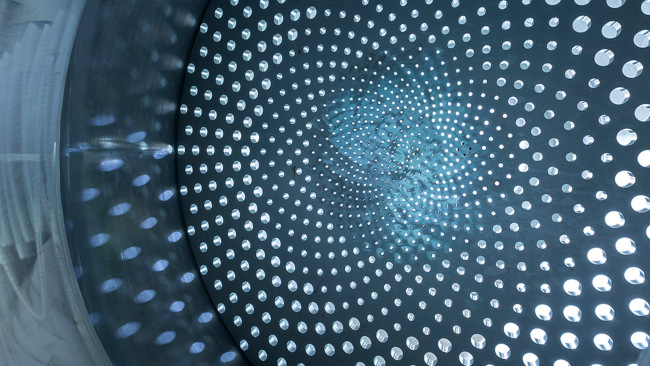
\includegraphics[height=0.6\textheight]{figures/photoexample-169}
\end{frame}


\section*{}

\begin{frame}{Conclusion}
  ...
\end{frame}

%\begin{frame}[c,plain]
\begin{frame}[c]
  \centering
  \Large Questions?
\end{frame}

\end{document}
